\documentclass{article}

%%% Functional packages
\usepackage{amsmath, amssymb, amsthm}
\usepackage{physics, siunitx}
\usepackage{isomath}        % for \vectorsym, \tensorsym, ...
\usepackage{textalpha}      % for upright Greek symbols
\usepackage{graphicx}
    \graphicspath{{pics/}}
\usepackage{subcaption}
\usepackage{multirow}
\usepackage{xspace}
\usepackage{minted}         % for listings
    \renewcommand{\listingscaption}{Listing}

%%% Configuration packages
%\usepackage{fullpage}
\usepackage{titlesec}

%%% TikZ
\usepackage{tikz}
\usetikzlibrary{shapes, arrows, chains}

\usepackage[
    pdfusetitle,
    colorlinks
]{hyperref}

\title{Thermal debinding}
\author{Oleg Rogozin}

%%% Bold symbols
\newcommand{\bv}{\vb*{v}}
\newcommand{\bn}{\vu*{n}}
\newcommand{\bx}{\vb*{x}}

%%% For algorithms
\newcommand{\V}{V}
\newcommand{\dV}{\partial V}
\newcommand{\intCell}{\int_{\V}}
\newcommand{\intFaces}{\oint_{\dV}\!\!\!\bn}
\newcommand{\implicit}[1]{\underbrace{#1}_\text{implicit}}
\newcommand{\explicit}[1]{\underbrace{#1}_\text{explicit}}
\newcommand{\OpenFOAM}{OpenFOAM\textregistered\xspace}

%%% For coloring
\usepackage{xcolor}
\newcommand{\alert}[1]{\textcolor{red}{#1}}

%%% Problem specific
\newcommand{\ResultsCaption}[2]{
    Simulation results of thermal debinding process for a cube
    with the side \SI{#1}{\mm} and the heating rate \SI{#2}{\celsius/\hour}.
    The following quantities versus temperature are shown:
    the mass fraction of the individual polymer components (a),
    maximum and minimum diffusion coefficient value (b),
    maximum density (c) and pressure (d) of the monomer.
    The monomer pressure is compared with the mechanical strength of the samples,
    measured experimentally.
    The gray area corresponds to the temperature interval in which samples are destroyed.
}

\begin{document}
\maketitle
\tableofcontents

\newcommand{\sectionbreak}{\clearpage}
\section{Mathematical model}\label{sec:td:model}

The government equation for monomer density is
\begin{equation}\label{eq:rho}
    \pdv{\rho}{t} + \div((D_1 + D_2)\grad\rho) = \phi_{p0}\dot{m},
\end{equation}
where $\dot{m} = -\rho_p\dot{y}$ is the source term,
\begin{equation}\label{eq:D1}
    D_1 = D_0e^{-E_d/RT}F(\psi_m,T)(1-\phi_c)^{3/2}
\end{equation}
is the diffusion coefficient, and
\begin{equation}\label{eq:D2}
    D_2 = \frac{Kp}{\mu_m\phi_m} = \frac{KRT}{\mu_mW_m\phi_m^2}\rho
\end{equation}
is the mass diffusivity due to gas convection.
The permeability is equal to
\begin{equation}\label{eq:K}
    K = \frac{d_c^2}{180}\alert{\qty(\frac{\phi_m}{1-\phi_c})^2}\frac{\phi_m^3}{(1-\phi_m)^2}.
\end{equation}

It is assumed that the molar mass of the monomer $W_m = \SI{100}{\g/\mol}$
and the characteristic size of a ceramic particle $d_c = \SI{e-7}{\m}$.

\section{Computational algorithm}

The numerical solution of the problem is based on the finite-volume method.
The system of equations described in section~\ref{sec:td:model} is discretized as follows:
\begin{gather}
    \implicit{\intCell \pdv{y_i}{t}} = -\implicit{\intCell k_iy_ie^{-E_i/RT}}, \label{eq:y_scheme}\\
    \implicit{\intCell \pdv{\rho}{t}} = \implicit{\intFaces \vdot((D_1+D_2)\grad\rho)}
        + \explicit{\sum_i\phi_{p0}\rho_p\intCell \pdv{y_i}{t} }, \label{eq:rho_scheme}
\end{gather}
where $\V$ is a control volume, $\dV$ is its boundary,
$\bn$ is the outward unit normal to $\dV$.
Curly bracket captions mean the type of discretization.
The equations~\eqref{eq:y_scheme} and~\eqref{eq:rho_scheme} are integrated using the Euler scheme,
while differential operators are approximated with the second-order accuracy in space. 
The global simulation flowchart is illustrated in Fig.~\ref{fig:td:flowchart}.

\begin{figure}[b!]
    \centering
    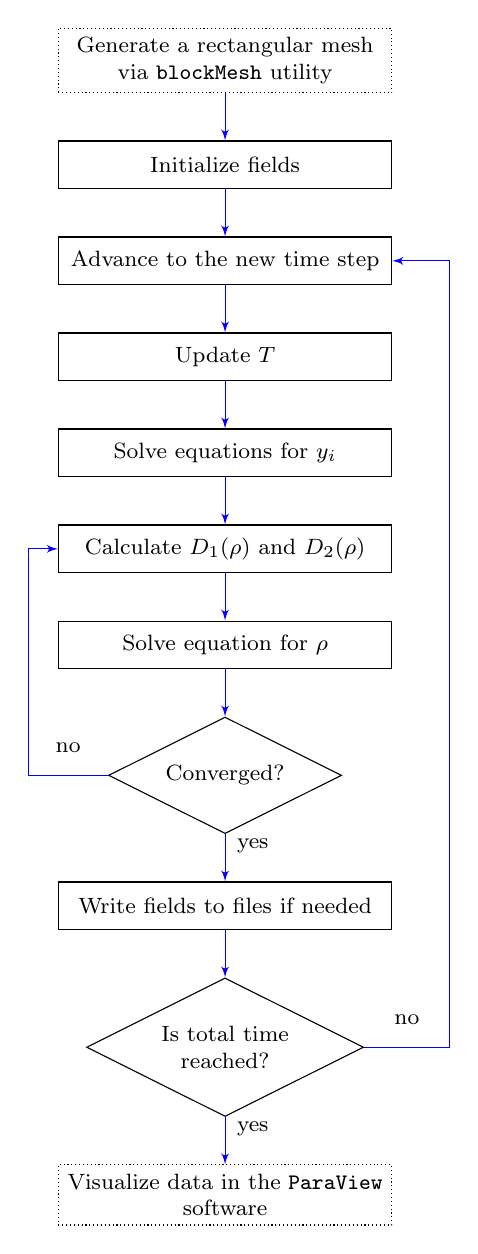
\begin{tikzpicture}[%
        >=latex',
        start chain=going below,    % General flow is top-to-bottom
        node distance=6mm and 60mm, % Global setup of box spacing
        every join/.style={norm},   % Default linetype for connecting boxes
        font=\footnotesize,         % \sffamily
    ]
    \tikzset{
        base/.style={draw, on chain, on grid, align=flush center, minimum height=4ex},
        proc/.style={base, rectangle, text width=4cm},
        util/.style={proc, densely dotted},
        test/.style={base, diamond, aspect=2, text width=5em},
        term/.style={proc, rounded corners},
        % coord node style is used for placing corners of connecting lines
        coord/.style={coordinate, on chain, on grid, node distance=6mm and 25mm},
        % nmark node style is used for coordinate debugging marks
        nmark/.style={draw, cyan, circle, font={\sffamily\bfseries}},
        % -------------------------------------------------
        % Connector line styles for different parts of the diagram
        norm/.style={->, draw, blue},
        free/.style={->, draw, green},
        cong/.style={->, draw, red},
        it/.style={font={\small\itshape}}
    }
    %%% Blocks
    \node [util] (first1) {
        Generate a rectangular mesh via \texttt{blockMesh} utility
    };
    \node [proc, join] {
        Initialize fields
    };
    \node [proc, join] (advance_time) {
        Advance to the new time step
    };
    \node [proc, join] {
        Update $T$
    };
    \node [proc, join] {
        Solve equations for $y_i$
    };
    \node [proc, join] (D) {
        Calculate $D_1(\rho)$ and $D_2(\rho)$
    };
    \node [proc, join] (rho) {
        Solve equation for $\rho$
    };
    \node [test, join] (conv_pimple) {Converged?};
    \node [proc, join] (write) {
        Write fields to files if needed
    };
    \node [test, join] (finish) {Is total time reached?};
    \node [util, join] (paraview) {
        Visualize data in the \texttt{ParaView} software
    };
    %%% Nodes
    \node [coord, left=of conv_pimple] (c4) {};
    \node [coord, right=of finish, xshift=1em] (c5) {};
    %%% Connectors
    % -- pimple
    \path (conv_pimple.south) to node [near start, xshift=1em] {yes} (write);
    \path (conv_pimple.west) to node [yshift=1em] {no} (c4);
        \draw [->,norm] (conv_pimple.west) -- (c4) |- (D);
    % -- time
    \path (finish.south) to node [near start, xshift=1em] {yes} (paraview);
    \path (finish.east) to node [yshift=1em] {no} (c5);
        \draw [->,norm] (finish.east) -- (c5) |- (advance_time);
    \end{tikzpicture}
    \caption{
        The global simulation flowchart.
        The dashed blocks correspond to the auxiliary utilities.
        The solid ones represent the procedures of the \texttt{thermalDebindingFoam}.
    }\label{fig:td:flowchart}
\end{figure}

\section{Implementation}

The described numerical algorithm is implemented as a developed \OpenFOAM solver.
Part of this implementation is presented as source code in listing~\ref{lst:debinding}.
The code enable calculations for arbitrary geometries using unstructured grids.
In addition, for complex geometries, it is possible to perform parallel multiprocessor computations.

\begin{listing}[b!]
    \footnotesize
    \begin{minted}{c++}
while (runTime.run() && gMax(T) < maxTemperature)
{
    ++runTime;

    Info<< "Time = " << runTime.timeName() << nl << endl;

    // --- Calculate the temperature
    T += heatingRate*runTime.deltaT();

    // --- Calculate the burning of polymer components
    forAllIter(PtrDictionary<polymerComponent>, polymer.components(), iter)
    {
        polymerComponent& y = iter();

        fvScalarMatrix yEqn
        (
            fvm::ddt(y) + fvm::Sp(y.degradationRate(T), y)
        );

        yEqn.solve(mesh.solverDict("massFraction"));
    }

    // --- Solve the transport equation for monomer
    while (pimple.loop())
    {
        D1 = polymer.diffusion(rho, T);
        p = polymer.pressure(rho, T);
        permeability = permeability0
            *pow(polymer.poresFraction()/polymer.totalVolumeFraction(), particleSizeExponent)
            *pow(polymer.poresFraction(), 3)/sqr(1 - polymer.poresFraction());
        D2 = permeability/mu/polymer.poresFraction()*p;
        D2.correctBoundaryConditions();

        fvScalarMatrix rhoEqn
        (
            fvm::ddt(rho) == fvm::laplacian(D1 + D2, rho)
        );

        forAllIter(PtrDictionary<polymerComponent>, polymer.components(), iter)
        {
            rhoEqn += polymer.initialVolumeFraction()*polymer.rho()*fvc::ddt(iter());
        }

        rhoEqn.solve();
    }

    runTime.write();
    runTime.printExecutionTime(Info);
}
    \end{minted}
    \caption{
        sample of the source code of \texttt{thermalDebindingFoam}
        for solving equations~\eqref{eq:y_scheme} and~\eqref{eq:rho_scheme}.
        The main computation loop is presented.
    }
    \label{lst:debinding}
\end{listing}

\section{Validation of the model}

%%% Simulation results
The process of thermal debinding was numerically modeled using the developed software component.
The results obtained for different samples (cubes of different sizes) and temperatures in the furnace are shown
in Fig.~\ref{fig:debinding_all_10mm_6KperHour}--\ref{fig:debinding_all_5mm_60KperHour}.

%%% Experimental strength data
Comparing the monomer pressure curve with experimentally measured strengths
of the sample gives an assessment of the probability of sample failure during thermal debinding.
In particular, the compressive, tensile, and flexural strengths of the samples
are shown in Fig.~\ref{fig:debinding_all_10mm_1KperHour}--\ref{fig:debinding_all_5mm_60KperHour}.
One can see that the samples are strengthened at \SI{200}{\celsius},
which probably associated with the removal of volatile components from the polymer mixture.
By the time the binder is completely removed (about \SI{400}{\celsius}),
the samples become particularly fragile.
Since the sample destruction due to monomer pressure corresponds to the tensile load,
it is necessary to compare the monomer pressure with this characteristic
in order to estimate the probability of failure.

%%%% Experimental observations of sample integrity
The validation of the developed model is based on the prediction of the fact of sample destruction,
as well as the temperature range in which this destruction occurs.
It is known from the experimental observations that a cube with the side \SI{10}{\mm}
breaks in the range $\SI{100}{\celsius}<T<\SI{200}{\celsius}$ for the heating rate \SI{6}{\celsius/\hour}.
In the same range, the cube with the side \SI{5}{\mm} is broken, but at \SI{60}{\celsius/\hour}.
This area is marked on the graphs with a gray background.
At lower heating rates, the samples retain their integrity.

%%% Comparison with them
In simulations, the maximum pressure is reached in the temperature range
from \SI{50}{\celsius} to \SI{200}{\celsius}
depending on the sample size and heating rate (see Table~\ref{table:tb:pressure}).
The data obtained are fully consistent with the experimental observations.
In particular, it can be seen that larger sample size leads to larger monomer pressure 
in the center of the sample due to an insufficient gas outlet,
which inevitably leads to its destruction.
Thus, printing parts with a thickness of the order \SI{10}{\mm} and more is challenging,
because it requires very slow heating, less than \SI{1}{\celsius/\hour}.
In addition, one can see that even thin-walled parts can break at high heating rate,
because the monomer has no enough time to leave the sample
and its pressure increases in proportion to the temperature.

%%% Second peak
The important peculiarity of the current simulations is the presence of the second peak
of monomer pressure, caused by the removal of the second polymer component
and observed at temperatures above \SI{200}{\celsius} for all cases
except Fig.~\ref{fig:debinding_all_10mm_60KperHour}.
Despite the fact that the second peak always turns out to be smaller in value than the first,
its role seems to be decisive in the formation of cracks in a part at later stages of thermal debinding,
when the sample loses its strength dramatically.

\begin{figure}
    \centering
    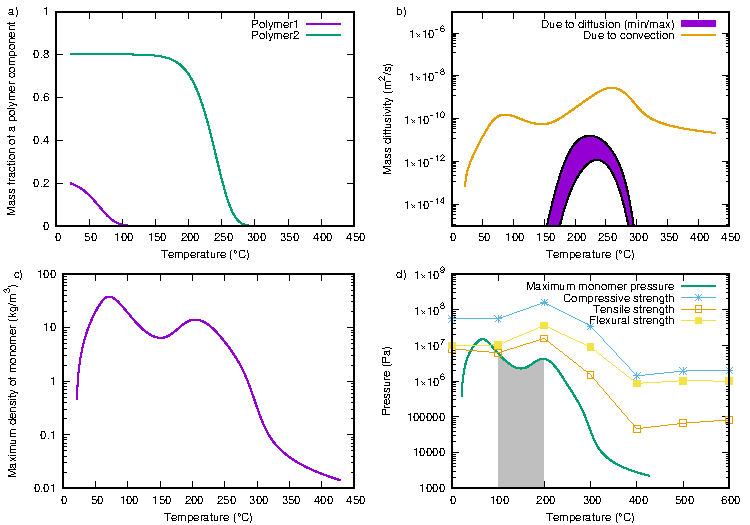
\includegraphics[width=\textwidth]{debinding_all_10mm_1KperHour}
    \caption{\ResultsCaption{10}{1}}
    \label{fig:debinding_all_10mm_1KperHour}
\end{figure}

\begin{figure}
    \centering
    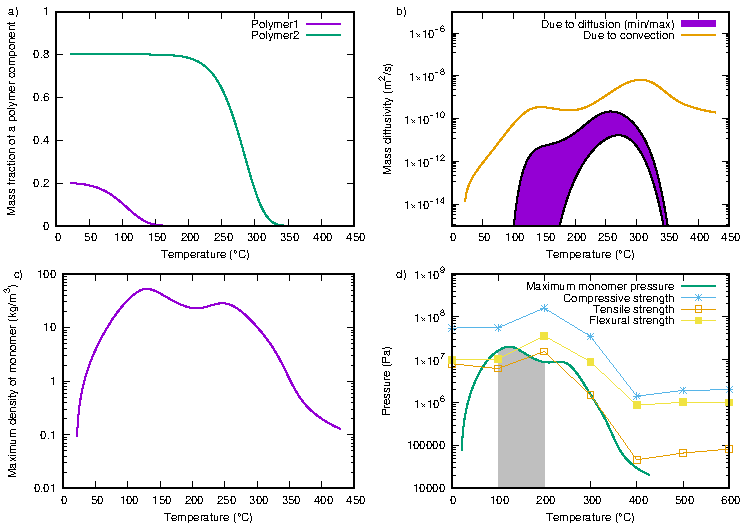
\includegraphics[width=\textwidth]{debinding_all_10mm_6KperHour}
    \caption{\ResultsCaption{10}{6}}
    \label{fig:debinding_all_10mm_6KperHour}
\end{figure}

\begin{figure}
    \centering
    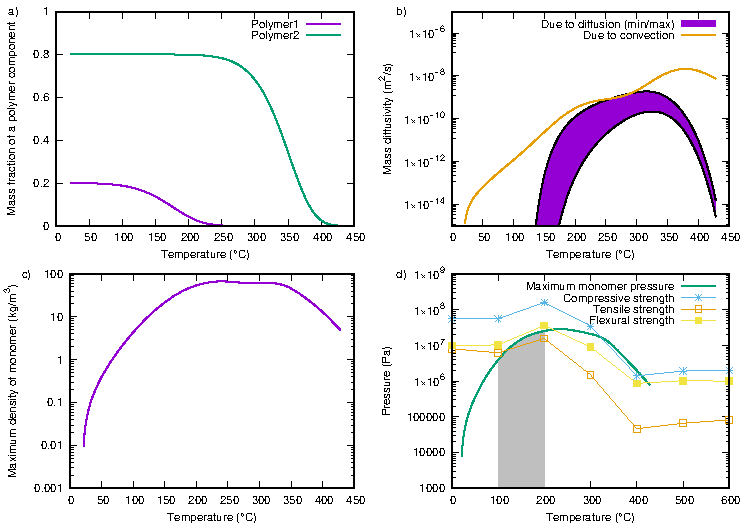
\includegraphics[width=\textwidth]{debinding_all_10mm_60KperHour}
    \caption{\ResultsCaption{10}{60}}
    \label{fig:debinding_all_10mm_60KperHour}
\end{figure}

\begin{figure}
    \centering
    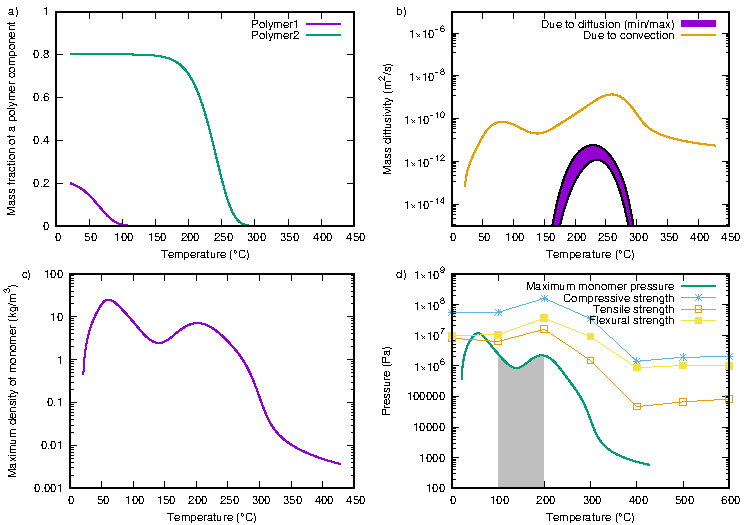
\includegraphics[width=\textwidth]{debinding_all_5mm_1KperHour}
    \caption{\ResultsCaption{5}{1}}
    \label{fig:debinding_all_5mm_1KperHour}
\end{figure}

\begin{figure}
    \centering
    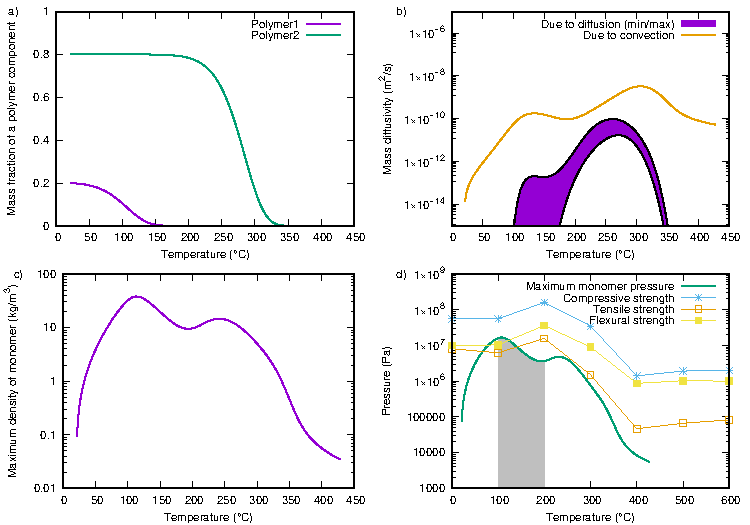
\includegraphics[width=\textwidth]{debinding_all_5mm_6KperHour}
    \caption{\ResultsCaption{5}{6}}
    \label{fig:debinding_all_5mm_6KperHour}
\end{figure}

\begin{figure}
    \centering
    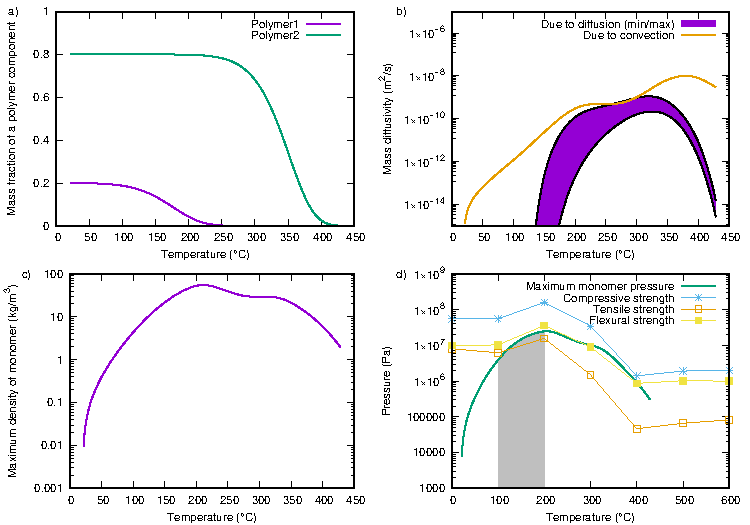
\includegraphics[width=\textwidth]{debinding_all_5mm_60KperHour}
    \caption{\ResultsCaption{5}{60}}
    \label{fig:debinding_all_5mm_60KperHour}
\end{figure}

\begin{table}
    \centering
    \caption{
        Maximum monomer pressure and temperature at which it was reached,
        obtained by numerical simulation of thermal debinding.
    }\label{table:tb:pressure}
    \centering
    \footnotesize
    \begin{tabular}{cccc}
        \hline
        Size of cube (\si{\mm}) & Heating rate (\si{\celsius/\hour})
            & Pressure (\si{\MPa}) & Temperature (\si{\celsius}) \\
        \hline
        10 & 1  & 14.9 & 67  \\
        10 & 6  & 20.3 & 125 \\
        10 & 60 & 28.5 & 235 \\
        5  & 1  & 11.6 & 57  \\
        5  & 6  & 16.7 & 108 \\
        5  & 60 & 24.9 & 205 \\
        \hline
    \end{tabular}
\end{table}


\end{document}
